% File: src/chapter_4_design.tex
% Project: Monitoring and Reporting Tool for Cloned Vulnerabilities across Open-Source Projects
% Author: Matus Remen (xremen01@stud.fit.vutbr.cz)
% Description: Chapter 4 - Design

\chapter{Design}
\label{chapter:design}
  This chapter presents the design of the proposed tool which, aims to address the challenges and requirements
  identified in the problem of detecting cloned vulnerabilities. It is organized into three main sections, each focusing
  on a~key aspect of the tool: architecture, workflow and user interface. These sections provide an overview
  of how the monitoring tool is structured, how it works, and how to interact with it.

  \section{Architecture}
  \label{section:architecture}
    In this section, the structural design of the tool is displayed. Presenting a~clear and organized
    view of its architecture, this section aims to demonstrate how various elements in the system work
    together to form a~coherent whole.

    Figure \ref{architecture} depicts the parts of this tool and the communication between them.
    The core of the application consists of the detection mechanism and its internal database. To interact
    with the core, it has available a~command line interface and a~web interface. The command line interface
    has direct access to the core of the tool, while the web is connected to the core via the application
    programming interface. All together builds a~tool offering two modes for detecting cloned vulnerabilities.
    The first one detects the propagation of a~specific vulnerability among the clones of the project where it was discovered.
    The second method discovers new flaws but is executable only from the command line.

    \bigskip

    \begin{figure}[h]
      \centering
      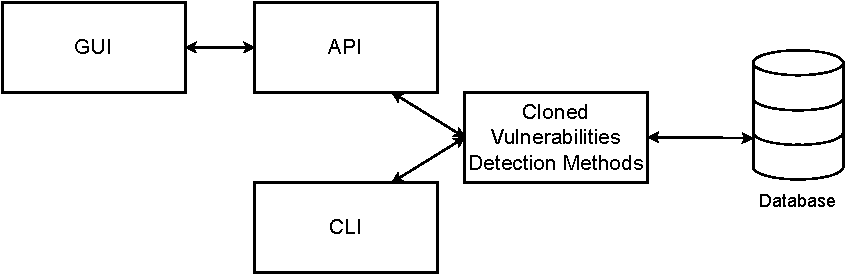
\includegraphics[width=0.95\textwidth]{obrazky-figures/architecture.drawio.pdf}
      \caption{Architecture of the tool.}
      \label{architecture}
    \end{figure}

    \subsection*{Database Schema of the Tool}
    \label{design:database}
    The database consists of two primary and one secondary entity set represented by an entity relation diagram
    in Figure~\ref{erd}. The primary entities contain configurations supporting the automation rate and scope
    of the detection mechanism. The secondary entity is used as a~container for vulnerability detection
    results and has no effect on the performance of the tool.

    The entity \texttt{Bug} contains details about vulnerabilities like an identifier in case of CVE, a~commit
    responsible for the repair of the bug, a~patch containing specific fix changes and a~code for particular
    methods for detecting clones. Depending on the configured method, if available, the patch is used
    by integration of BlockScope described in Section~\ref{section:blockscope}. While the value in attribute \texttt{code}
    would be used by an integrated clone detection tool Simian\footnote{\href{https://devel.nuclex.org/external/svn/simian/trunk/index.html}
    {https://devel.nuclex.org/external/svn/simian/trunk/index.html}}.
    Additionally, this entity contains attribute \texttt{verified} to inform about whether the bug was reviewed
    by an administrator as all records in this table are created automatically during the run of the detection
    method. Firstly, in the case of CVE records, the vulnerability databases do not always refer explicitly
    to the specific fix commit or patch, but it is detected by various scans which will be mentioned in the next
    Section \ref{section:workflow}. Secondly, the application programming interface (API) of the National Vulnerability
    Database~\ref{section:nvd} has a~limited availability of five queries per rolling thirty seconds time window\footnote{
    \href{https://nvd.nist.gov/developers/start-here}{https://nvd.nist.gov/developers/start-here} -- rate limits}.
    Storing and reusing previously requested data prevents from reaching the query limit and allows to subsequently
    further edit and specify particular details, so the tool can process them faster and run smoother.
    Lastly, the attribute \texttt{created} contains a~timestamp of record creation, which represents scan times.
    The repositories can be updated over time and older scans might not be relevant since new commits were released
    and the identified bugs could be fixed. The relation \texttt{discovered in} binds a~bug to the project where it was found.
    Overall, the~attributes of this entity support the performance of the tool and allow it to run automatically
    skipping the~step of the manual selection of the relevant patch code.

    On the other hand, the entity set \texttt{Project} not only offers performance benefits but also contains important
    data related to the configuration of the workflows. The attribute \texttt{url} contains a~link used for initialization
    of the repositories by cloning to a~fresh environment of the tool, after adding a~new project or basically
    when it is missing. Attribute \texttt{name} and~\texttt{author} are used mainly for easier referencing from user input
    and logs. The \texttt{language} contains the programming language of the project for filtering the relevant
    files and code in the repository. The value of attribute \texttt{watch} marks projects which are updated and checked
    daily for potential vulnerability patching commits. Lastly, the timestamp in the attribute \texttt{added}, informs
    about the time of registration. The relation \texttt{forked by} models the~hierarchy of parent and cloned projects
    which are used in the detection methods to~decide which projects are potentially affected by a~cloned vulnerability.
    Accordingly, the detection is performed only among them. The records in this table are created on demand during
    the process of project registration.

    Lastly, the entity set \texttt{Detection} represents only positive results of detection methods which form a~relation
    between bugs and forked projects. Additionally, it also provides confidence in the result and the timestamp.
    Confidence is a number in the range of 0.0 -- 2.0, which represents the similarity of patch code and target code.
    Information from these entities does not affect the tool but serves as a~storage of results from previous scans.
    Consequently, the results can be cross-checked, and the maintainers of~affected projects can be notified about the presence
    of the cloned vulnerability.

    \begin{figure}[h]
      \centering
      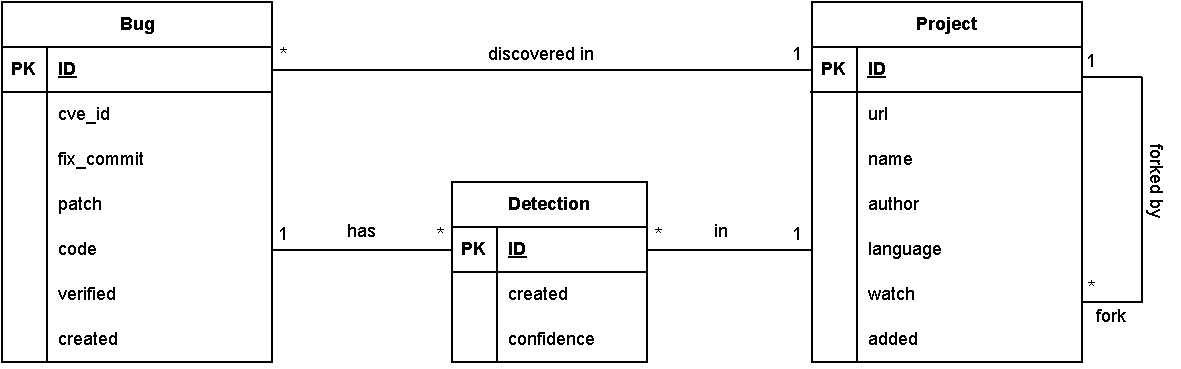
\includegraphics[width=0.95\textwidth]{obrazky-figures/cloneguard_erd.drawio.pdf}
      \caption{Entity relation diagram.}
      \label{erd}
    \end{figure}
    \bigskip

  \section{Workflow of the Detection Mechanisms}
  \label{section:workflow}
  As already mentioned in the previous section, the tool has two modes for detecting cloned vulnerabilities.
  The process of the first mode is similar to the CoinWatch and BlockScope. The second one
  performs periodic scans of parent repositories with an attempt to detect new potential
  flaws from recent patch commits. This functionality extends the detection options of the mentioned tools.

  \subsection*{Targeted Detection}
  \label{section:targeted-detection}
  The workflow of the targeted detection is displayed in~the~Figure~\ref{cg-workflow1}.
  It is executed on demand and requires an input, which contains a~reference to~vulnerability and the name of the project
  where it was discovered. It is mandatory for the project to be registered in the database prior to the vulnerability detection scan, so the mechanism
  has available all the required information about it.

  If the requirements are met, the detection mechanism starts with collecting information about the provided weakness
  and~initializes the repository of the target project. Firstly, the tool checks whether the provided reference
  to the vulnerability is available in the internal database. Otherwise, if CVE ID was provided the tool fetches
  its data using a vulnerability identifier from NVD using their API and stores the response in a~cache. Consequentially,
  based on the fetched
  data the patch commit is searched in the target repository. Afterwards, if it was not in the internal database
  before, it is stored here. If the search found multiple candidate commits or one is very extensive, the user
  is requested to specify the patch commit and code that is responsible for fixing the~vulnerability to reduce the number
  of candidates. This input is accordingly stored in the created record in the database.

  In the next step, all registered forks of the target project are initialized. That means if~their repositories
  are missing in the local storage of the tool, they will be cloned using attribute \texttt{url} of entity \texttt{Project}.
  In case they are downloaded, they are updated by pulling changes from their remote repository.
  It is also possible to~configure the tool to downgrade the repositories to an older version, which will be utilized
  in experimentation with the tool.
  This can be achieved by providing a~specific date in the input of the tool. In that case, the last commit
  before the~provided date will be selected and the repository will be reverted to that particular commit.

  At this point, all potentially affected projects are prepared for further investigation of~possible
  propagation of the vulnerability during forking or preliminary fetching. In the default setup, a~detection
  method based on the approach presented in the research paper about BlockScope is used~\cite{BlockScope}. Firstly,
  the surrounding code chunks -- contexts are fetched from fixing commit or directly from specific patch code
  present in attribute \texttt{patch} in the database. The~patch contexts are then searched for in the prepared
  set of repositories based on the code similarity. The detected contexts and the code in between then produce
  candidate code chunks, which are in the end compared to the patch code. In the end, based on the similarity
  of the patch and candidate code, the tool determines whether the patch was applied and so whether the weakness
  was fixed~\cite{BlockScope}. Alternatively, it is possible to configure using the tool Simian for the detection
  of clones, but in this case, it is mandatory to specify the code that should be detected among the forked repositories.
  Although, against the default method, Simian lacks the ability to detect Type~II and Type~III clones.
  Finally, after scanning a~project the positive detection results are stored in the database in table \texttt{Detection}.

  \begin{figure}[h]
    \centering
    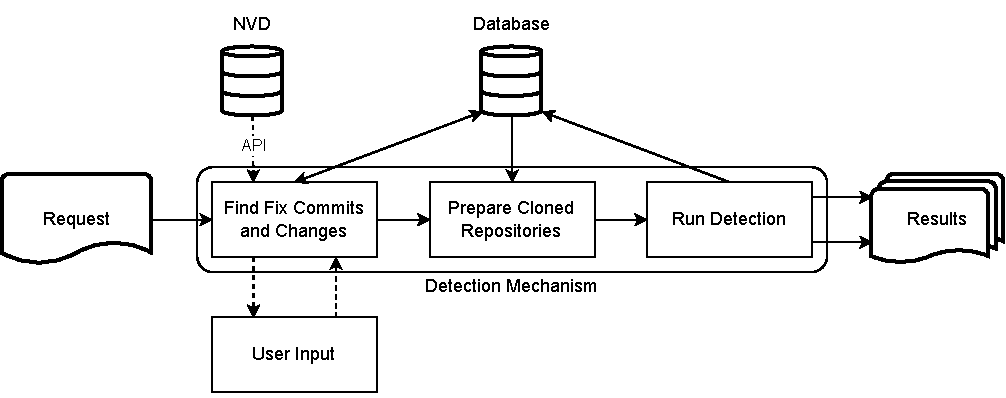
\includegraphics[width=0.95\textwidth]{obrazky-figures/cloneguard_workflow1.drawio.pdf}
    \caption{Basic workflow of the targeted detection scan.}
    \label{cg-workflow1}
  \end{figure}

  \subsection*{Discovery Scan}
  The workflow of the discovery scan is visible in Figure~\ref{cg-workflow2}. It is designed to run in schedules mainly.
  The goal of this mode is to detect new suspicious commits in monitored repositories which might imply
  new vulnerabilities in forked projects.

  On execution, the watched projects are fetched from the database and their repositories are updated to the latest
  version from the remote server using git. The messages of the latest commits are then scanned for the presence
  of any keyword from a~set containing CWE names\footnote{\href{https://cwe.mitre.org/data/definitions/1387.html}{https://cwe.mitre.org/data/definitions/1387.html} -- top 25 most dangerous weaknesses in 2022}.
  Secondly, a~check of affected files by a~commit is performed based on the file extension and path. For example, changes
  in documentation, release notes and tests are filtered out.

  After applying the filters, the resulting list of commits is reported via e-mail notification for each project,
  stored in the database and passed for further evaluation. The goal of the evaluation is to determine
  the complexity of the patch from each commit based on its granularity and spread. The complexity is represented by the number
  of extracted contexts from a~patch. The ones with low complexity
  can be processed automatically, so they are passed to the detection mechanism. In the end, the results
  are stored in the database and are observable in the logs or presented in the web interface.

  \begin{figure}[h]
    \centering
    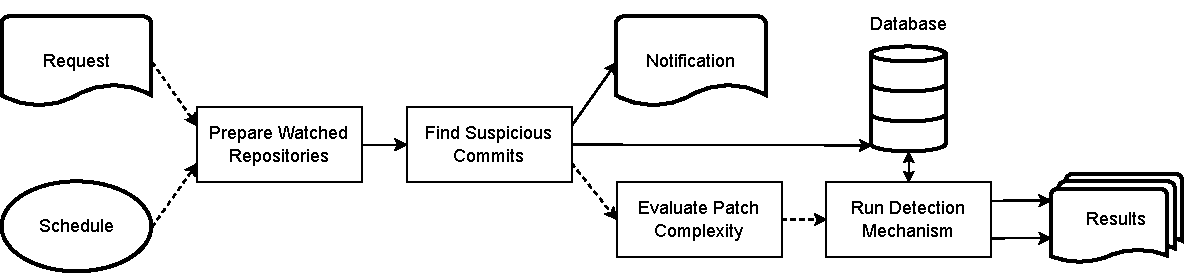
\includegraphics[width=0.95\textwidth]{obrazky-figures/cloneguard_workflow2.drawio.pdf}
    \caption{Workflow of the scheduled vulnerability scan.}
    \label{cg-workflow2}
  \end{figure}

  \section{User Interface}
  \label{design:ui}
  To enhance the user experience and improve overall effectiveness, the tool offers a~graphical interface alongside
  the command line interface. This section will contain a~graphical design of both interfaces, explaining the design choices
  and describing their functionality and use cases. Well designed user interface improves the overall experience with the tool,
  so it is crucial to present the results conveniently.

  \subsection*{Web}
  The graphical user interface (GUI) is accessible via a~web that communicates with the core of the tool
  using an application programming interface (API).
  The web page is organized into three crucial pages. The initial page presents an overview of the current state of the tool.
  Subsequently, a~user can navigate to the second page to initiate and configure the detection process.
  The third page showcases the detection results enabling the user to efficiently analyse and interpret the outcome.
  Additionally, using the tab in the upper right corner user can navigate to the documentation of the API.

  The draft of the page containing an overview of the tool is displayed in Figure~\ref{cg-web-overview}.
  It allows a~user to observe the state of the database, namely registered repositories and stored vulnerability
  records. As was mentioned in the Subsection~\ref{section:targeted-detection}, only registered repositories can be scanned
  by the detection method. Here it is possible to register new repositories to the tool by providing an URL,
  the programming language and the parent of the project in case it was forked from one of the already registered projects. In the second table, the records of previously
  scanned vulnerabilities can be updated to improve the precision and performance of the detection method.
  After updating a~record of the vulnerability it becomes marked as verified. This marking is visible in the last attribute
  of the entity.

  Figure~\ref{cg-web-search} displays the page, where the detection can be started after providing the required
  parameters -- identification of the vulnerability and its source project for the targeted detection.
  The identification of the vulnerability refers to the one stored in the internal database. The parameter \texttt{date}
  is optional. The first step of the detection method is executed using the button \texttt{Search}.
  Accordingly, the results from the search of fix commits are shown below. The list of candidate fix commits is observable
  on the left side of the page. After selecting a~specific commit, the changes from the commit are displayed in the adjacent
  text area. In order to start the clone detection, optionally the patch or code in the middle
  of the page can be edited to contain only code relevant to the fix of the vulnerability. Whether a~patch or code
  segment is required depends on the method which should be used for the detection of clone propagation. In case the search
  is done for a~known and verified vulnerability in the internal database, the stored values are pre-filled in the input
  fields. The button \texttt{Detect} then starts the clone detection.

  \begin{figure}[h]
    \centering
    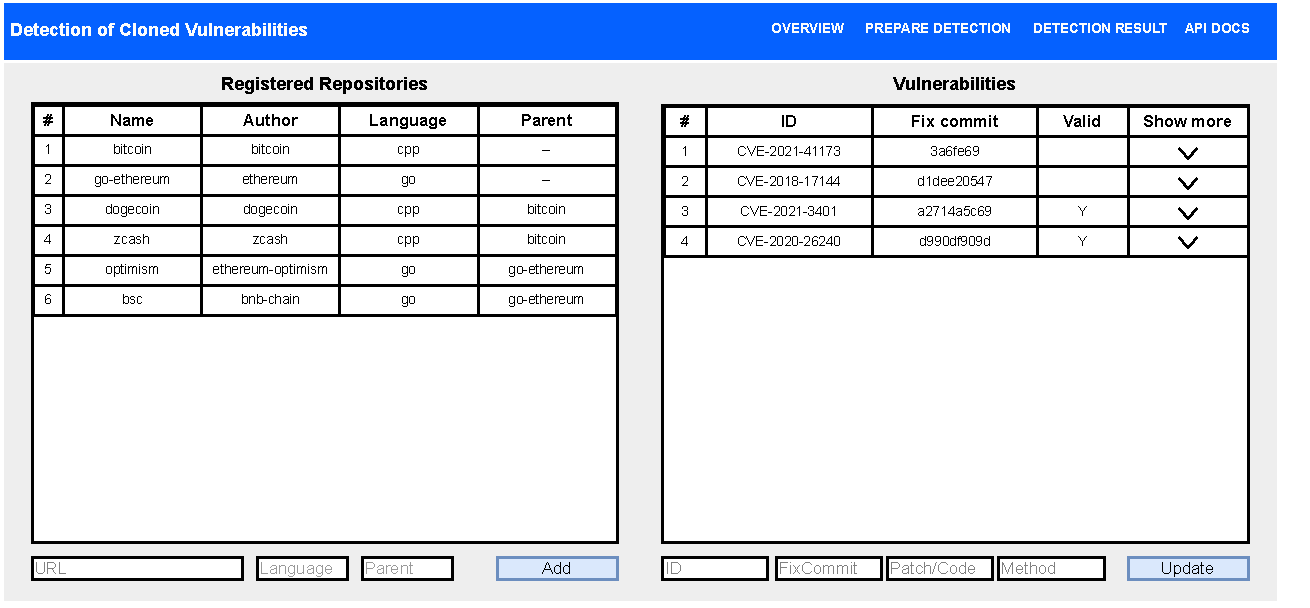
\includegraphics[width=0.95\textwidth]{obrazky-figures/cg_web_overview.drawio.pdf}
    \caption{The design of the page displaying an overview of the state of the tool.}
    \label{cg-web-overview}
  \end{figure}

  \begin{figure}[h]
    \centering
    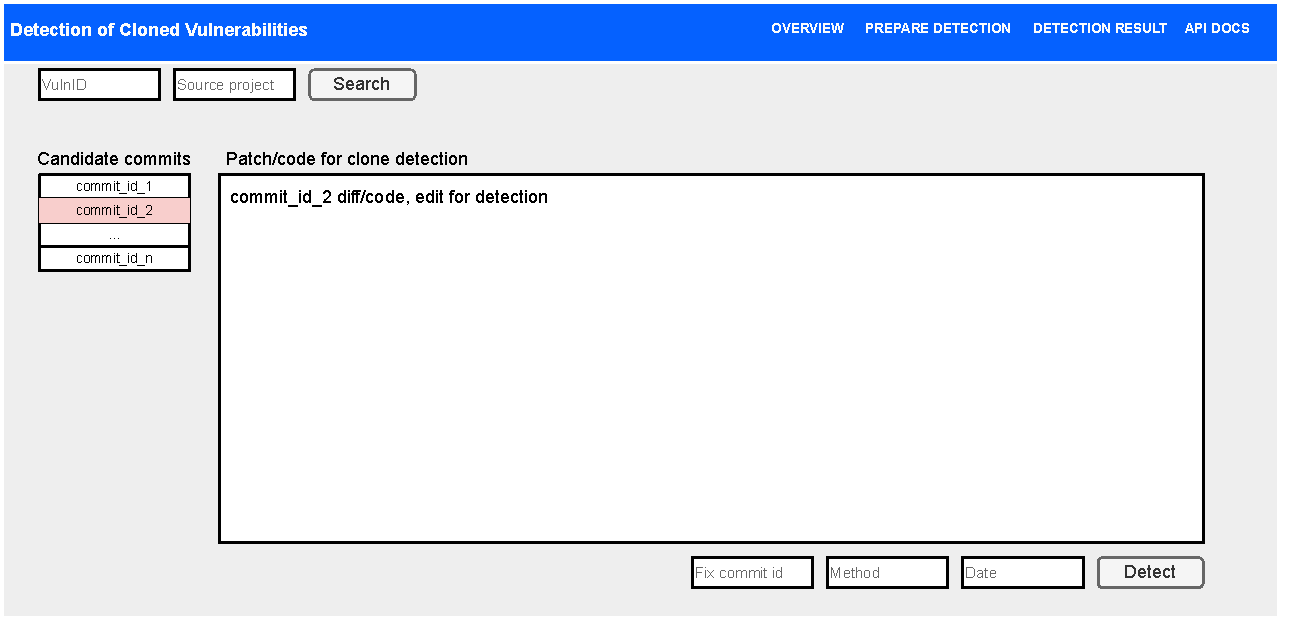
\includegraphics[width=0.95\textwidth]{obrazky-figures/cg_web_search.drawio.pdf}
    \caption{The design of the page where the detection mechanism can be configured and started.}
    \label{cg-web-search}
  \end{figure}

  After the detection is started, the logs and the preliminary results are visible on the last page. The design of this
  page is pictured in Figure~\ref{cg-web-results}. The page is just informative and does not affect the detection.
  The logs contain everything connected to the detection algorithm and the actual results can be hardly visible. To improve the transparency of the results,
   a~list containing a~summary of the detected cloned vulnerabilities is located on the right side. It provides the name of
  the affected project, the confidence of the result and a~reference to the location of the clone in the directory of the project.

  \begin{figure}[h]
    \centering
    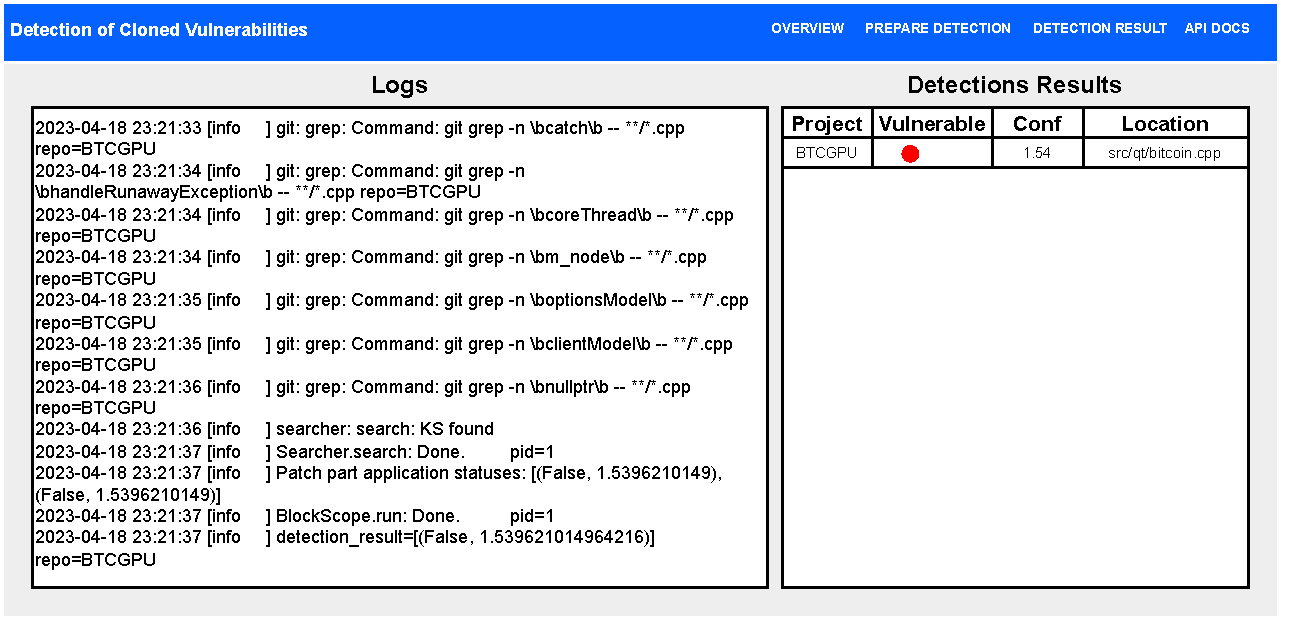
\includegraphics[width=0.95\textwidth]{obrazky-figures/cg_web_results.drawio.pdf}
    \caption{The design of the page displaying the logs and positive detection results.}
    \label{cg-web-results}
  \end{figure} % TODO: location of the candidate

  \subsection*{Command Line Interface}
  The command line interface (CLI) is a~fundamental way to interact with the tool. In comparison to the GUI,
  it offers advantages in terms of speed, customizing and automation. The functionalities allow a~user to:
  \begin{itemize}
    \item register new projects
    \item run the targeted detection
    \item configure schedule of the discovery scan
    \item run a~discovery scan
    \item initialize the schema of the internal database
  \end{itemize}

  In addition to the GUI capabilities, the CLI offers configuration and execution of discovery scan, initialization
  and execution of tests of the detection method. Unlike the GUI, which relies on communication using API, the CLI interacts
  directly with the core of the tool. This dual interface design caters to diverse user preferences, enhancing the overall
  user experience and functionality of the tool.
